\chapter{Desarrollo del Proyecto}
\label{anx:desarrollo}

\section{Sprint 1 (Hitos 1–4)}

\subsection{Planificación del Sprint 1}

\subsubsection{Objetivo y fechas}
El Sprint 1 se planificó del 29/09/2026 al 27/10/2026 con el objetivo de entregar la base de una aplicación SaaS con gestión de usuarios, arquitectura en capas, proceso Scrum en DoneTonic, flujo GitHub Flow, integración y despliegue continuos (CI/CD) en Google Cloud Run y Render, y una batería de pruebas automatizadas. El alcance formal, según directriz docente, se limitó inicialmente a los Hitos 1, 2 y 3 del enunciado (documentacion-tecnica.md §2.3).

\subsubsection{Sprint Backlog}
El Product Backlog inicial contenía 15 PBIs (P1–P14, P18) correspondientes a los Hitos 1–3. Durante el sprint se añadió el PBI \textbf{P19} (despliegue en Google Cloud Run) tras la concesión de créditos educativos de Google Cloud, elevando el total a 16 PBIs en el alcance de la entrega (gestion/README.md §4.1). La Tabla \ref{tab:sprint1-backlog} muestra el sprint backlog con sus hitos y estado final.

\begin{longtable}{@{}L{0.7cm} L{1.0cm} L{7.5cm} L{2.2cm}@{}}
\caption{Sprint Backlog del Sprint 1 (19 PBIs, 16 en alcance de entrega).}\label{tab:sprint1-backlog}\\
\toprule
\textbf{PBI} & \textbf{Hito} & \textbf{Título} & \textbf{Estado} \\ \midrule \endfirsthead
\toprule
\textbf{PBI} & \textbf{Hito} & \textbf{Título} & \textbf{Estado} \\ \midrule \endhead
P1 & H1 & Repositorio GitHub y flujo GitHub Flow & Hecho \\
P2 & H1 & Integración continua (CI) & Hecho \\
P3 & H1 & Despliegue continuo en URL pública & Hecho \\
P4 & H1 & Lógica de gestión de usuarios (en memoria) & Hecho \\
P5 & H1 & Pruebas unitarias automatizadas de la lógica & Hecho \\
P6 & H1 & Capa API de usuarios & Hecho \\
P7 & H2 & Frontend: interfaz y cliente de comunicación separados & Hecho \\
P8 & H2 & Registro e inicio de sesión locales & Hecho \\
P9 & H2 & Cierre de sesión y mantenimiento de la sesión & Hecho \\
P10 & H2 & Rutas protegidas en el servidor & Hecho \\
P11 & H3 & Persistencia en base de datos real & Hecho \\
P12 & H3 & Gestión de secretos con variables de entorno & Hecho \\
P13 & H3 & Roles de usuario y administrador & Hecho \\
P14 & H3 & Registro (log) de la actividad & Hecho \\
P15 & H4 & Inicio de sesión con proveedor externo (OAuth) & Hecho \\
P16 & H4 & Confirmación de cuenta por correo electrónico & Hecho \\
P17 & H4 & Manejo de errores y feedback al usuario & Hecho \\
P18 & H4 & README completo y revisión de la entrega & Hecho \\
P19 & H4 & Despliegue continuo en Google Cloud Run & Hecho \\
\bottomrule
\end{longtable}

Como se ve en la Tabla \ref{tab:sprint1-backlog}, todos los PBIs finalizaron en estado \textit{Hecho}.

\subsubsection{Historias de usuario y criterios de aceptación (Sprint 1)}
Los PBIs del Sprint 1 derivan directamente de los requisitos del enunciado; cada uno tiene su historia de usuario y criterios en DoneTonic. Por brevedad, se remite a \texttt{docs/gestion/README.md} (sección «Sprint 1: backlog, trazabilidad y evolución») donde se listan los 19 PBIs con sus títulos.

\subsubsection{Trazabilidad}
Cada PBI se desglosó en 1–2 tareas técnicas (T1–T32), cada una con su rama \texttt{hito-N/Tx-descripcion}, pull request \texttt{[Tx] ...} hacia \texttt{hito-N/integracion} y fusión tras CI en verde. Los cierres de hito fueron PR \#9 (Hito 1), \#17 (Hito 2), \#24 (Hito 3), \#29 (cierre sprint) y \#32 (revisión final). La trazabilidad completa tarea → rama → PR figura en \texttt{docs/gestion/README.md} y en la Tabla \ref{tab:sprint1-trazabilidad} (tareas de los 19 PBIs).

{\small
\begin{longtable}{@{}L{0.7cm} L{1.0cm} L{5.5cm} L{3.5cm} L{2.5cm}@{}}
\caption{Trazabilidad tarea → PR del Sprint 1 (32 tareas).}\label{tab:sprint1-trazabilidad}\\
\toprule
\textbf{PBI} & \textbf{Tarea} & \textbf{Descripción} & \textbf{PR} & \textbf{Estado} \\ \midrule \endfirsthead
\toprule
\textbf{PBI} & \textbf{Tarea} & \textbf{Descripción} & \textbf{PR} & \textbf{Estado} \\ \midrule \endhead
P1 & T1 & Crear repositorio y estructura base & \#1 & Hecho \\
P1 & T2 & Configurar GitHub Flow & \#2 & Hecho \\
P2 & T3 & Workflow de CI con GitHub Actions & \#3 & Hecho \\
P3 & T4 & Despliegue automático en proveedor cloud & \#4, \#10 & Hecho \\
P4 & T5 & Modelo de usuario y repositorio en memoria & \#5 & Hecho \\
P4 & T6 & Servicio de gestión de usuarios & \#6 & Hecho \\
P5 & T7 & Framework de pruebas y al menos 5 pruebas & \#7 & Hecho \\
P6 & T8 & Endpoints de la API de usuarios & \#8 & Hecho \\
P7 & T9 & Cliente de comunicación con la API & \#11 & Hecho \\
P7 & T10 & Interfaz de usuario: vistas y navegación & \#12 & Hecho \\
P8 & T11 & Registro y login en el backend (con hash) & \#13 & Hecho \\
P8 & T12 & Formularios de registro y login en el frontend & \#14 & Hecho \\
P9 & T13 & Mantener la sesión al recargar y cerrar sesión & \#15 & Hecho \\
P10 & T14 & Middleware de autenticación y protección de rutas & \#16 & Hecho \\
P11 & T15 & Elegir y configurar la base de datos & \#18 & Hecho \\
P11 & T16 & Repositorio de BD sustituyendo al de memoria & \#19 & Hecho \\
P12 & T17 & Sacar los secretos a variables de entorno & \#20 & Hecho \\
P13 & T18 & Roles, autorización y primer administrador & \#21 & Hecho \\
P13 & T19 & Panel de administración y baja de cuenta & \#22 & Hecho \\
P14 & T20 & Configurar el logging de la actividad relevante & \#23 & Hecho \\
P15 & T21 & Registrar la aplicación OAuth en Google & \#40 & Hecho \\
P15 & T22 & Flujo de inicio de sesión con OAuth & \#40 & Hecho \\
P16 & T23 & Servicio de correo & \#38 & Hecho \\
P16 & T24 & Flujo de confirmación de la cuenta & \#39 & Hecho \\
P17 & T25 & Errores en el backend & \#37–\#41 & Hecho \\
P17 & T26 & Mensajes de error en el frontend & \#37–\#41 & Hecho \\
P18 & T27 & Completar el README & \#25 & Hecho \\
P18 & T28 & Etiquetas de hito y revisión final & \#26 & Hecho \\
P18 & T31 & Revisión frase a frase contra el enunciado & \#30 & Hecho \\
P18 & T32 & Carpeta de la memoria en LuaLaTeX & \#31 & Hecho \\
P19 & T29 & Contenerizar la aplicación con Docker & \#27 & Hecho \\
P19 & T30 & Despliegue continuo en Cloud Run con GitHub Actions & \#28 & Hecho \\
\bottomrule
\end{longtable}
}

La Tabla \ref{tab:sprint1-trazabilidad} resume la correspondencia entre cada tarea y su pull request.

\subsection{Desarrollo del Sprint 1: problemas y soluciones}

Los problemas técnicos surgidos y sus soluciones, extraídos de la documentación del proyecto (documentacion-tecnica.md §13), se resumen en las Tablas \ref{tab:prob-desarrollo} a \ref{tab:prob-donetonic}.

\begin{longtable}{@{}L{5.5cm} L{8.5cm}@{}}
\caption{Problemas y soluciones en desarrollo y pruebas.}\label{tab:prob-desarrollo}\\
\toprule
\textbf{Problema detectado} & \textbf{Solución adoptada} \\ \midrule \endfirsthead
\toprule
\textbf{Problema detectado} & \textbf{Solución adoptada} \\ \midrule \endhead
\texttt{pg-mem} no admitía \texttt{CREATE TABLE IF NOT EXISTS} ni funciones de sesión & Consulta a \texttt{information\_schema}; prueba de sesiones solo contra PostgreSQL real en CI \\
Cookie \texttt{secure} no guardada en local con \texttt{NODE\_ENV=production} sobre HTTP & Comportamiento esperado por seguridad; capturas locales en modo desarrollo \\
\texttt{pkill -f "node src/server.js"} cerraba la shell invocadora & Arranque del proceso de servidor con \texttt{setsid} desde script \\
Tabla de administración no cabía en 640~px; botón \textit{Eliminar} oculto & Contenedor ampliado; en móvil, cada usuario se muestra como tarjeta (Fig. \ref{fig:app-admin-movil}) \\
Capturas Playwright en GitHub salían sin estilos por recursos bloqueados & Descartadas; capturas de la propia aplicación generadas correctamente \\
Docker Hub bloqueado en entorno en la nube & Simulación local (\texttt{npm ci --omit=dev}); validación real en job del CI \\
JSON mal formado devolvía HTML de Express & Manejador propio tras parser: 400 JSON en toda la API (prueba técnica) \\
Correo no salía desde Cloud Run (puerto 25/587 bloqueado) & SMTP Gmail puerto 465 con contraseña de aplicación en Secret Manager \\
\texttt{redirect\_uri\_mismatch} en Google OAuth & Registrar las dos URLs de Cloud Run y localhost en cliente Google; usar \texttt{PUBLIC\_URL} \\
Ramas Hito 4 dependían unas de otras & Reubicar (rebase) sobre \texttt{main} real antes de abrir PRs, cada una con CI verde \\
\bottomrule
\end{longtable}

\begin{longtable}{@{}L{5.5cm} L{8.5cm}@{}}
\caption{Problemas y soluciones en despliegue Google Cloud.}\label{tab:prob-despliegue}\\
\toprule
\textbf{Problema detectado} & \textbf{Solución adoptada} \\ \midrule \endfirsthead
\toprule
\textbf{Problema detectado} & \textbf{Solución adoptada} \\ \midrule \endhead
Script preparación falló en Artifact Registry por propagación IAM & Reejecución parametrizada con \texttt{PROJECT\_ID}; script idempotente \\
Secreto \texttt{database-url} mal introducido en Cloud Run & Nueva versión del secreto (v2) con \texttt{gcloud secrets} \\
URL pública Cloud Run devolvía 404 & Primer despliegue pendiente; operativa tras finalizar workflow \\
Cadena de conexión Neon compartida en chat & Recomendación rotar clave; aplazada en lista de tareas pendientes \\
\bottomrule
\end{longtable}

\begin{longtable}{@{}L{5.5cm} L{8.5cm}@{}}
\caption{Problemas y soluciones en Git y GitHub.}\label{tab:prob-git}\\
\toprule
\textbf{Problema detectado} & \textbf{Solución adoptada} \\ \midrule \endfirsthead
\toprule
\textbf{Problema detectado} & \textbf{Solución adoptada} \\ \midrule \endhead
\texttt{git push --all} rechazado en ramas integración (non-fast-forward) & Sincronización mediante \texttt{git fetch} y \texttt{git branch -f} \\
Entorno cloud sin permisos escritura directa en GitHub & Exportación commits vía \texttt{git bundle}; push desde local \\
Bundle requería commit base ausente en repo local & Regeneración tomando base commit 4b16182 (16182) \\
Subida bundle con mismo nombre sobrescribía versión anterior & Asignación nombres de fichero unívocos \\
Fusiones en interfaz web fallaban por comprobaciones incompletas & Espera a validación checks y confirmación explícita \\
\bottomrule
\end{longtable}

\begin{longtable}{@{}L{5.5cm} L{8.5cm}@{}}
\caption{Problemas y soluciones en alcance y revisión.}\label{tab:prob-alcance}\\
\toprule
\textbf{Problema detectado} & \textbf{Solución adoptada} \\ \midrule \endfirsthead
\toprule
\textbf{Problema detectado} & \textbf{Solución adoptada} \\ \midrule \endhead
Requisitos OAuth y confirmación correo pertenecientes a Hito 4 & Alcance limitado a Hitos 1–3 por docente; código guardado \\
Endpoint \texttt{/api/users/:id/active} accesible a usuarios estándar & Restricción exclusiva a rol administrador (PR \#30) tras revisión \\
Documentos de revisión redactados a partir de PBIs y no del PDF & Reescritura sistemática de \texttt{docs/revision-entrega.md} \\
\bottomrule
\end{longtable}

\begin{longtable}{@{}L{5.5cm} L{8.5cm}@{}}
\caption{Problemas y soluciones en memoria LaTeX.}\label{tab:prob-latex}\\
\toprule
\textbf{Problema detectado} & \textbf{Solución adoptada} \\ \midrule \endfirsthead
\toprule
\texttextbf{Problema detectado} & \textbf{Solución adoptada} \\ \midrule \endhead
Error escritura auxiliares en subcarpetas al compilar en \texttt{build/} & Configuración \texttt{.latexmkrc} con creación recursiva directorios \\
Ausencia librerías LuaLaTeX en entorno pruebas & Instalación dependencias; compilación validada en GitHub Actions \\
\bottomrule
\end{longtable}

\begin{longtable}{@{}L{5.5cm} L{8.5cm}@{}}
\caption{Problemas y soluciones en DoneTonic.}\label{tab:prob-donetonic}\\
\toprule
\textbf{Problema detectado} & \textbf{Solución adoptada} \\ \midrule \endfirsthead
\toprule
\textbf{Problema detectado} & \textbf{Solución adoptada} \\ \midrule \endhead
Menús apilados y clics JS ineficaces en interfaz Flutter & Automatización por coordenadas comprobando árbol accesibilidad \\
Renderizado distorsionado al forzar tamaño ventana en Flutter & Capturas realizadas con resolución nativa de 800~px \\
\bottomrule
\end{longtable}

Las Tablas \ref{tab:prob-desarrollo} a \ref{tab:prob-donetonic} recogen la resolución de incidencias sin formato de diario.

\subsection{Revisión del Sprint 1}

Al cierre del Sprint 1 (27/10/2026, commit final, PR \#32 y posteriores) se entregaron:
\begin{itemize}
    \item Cinco releases publicadas en GitHub: \texttt{hito-1}, \texttt{hito-2}, \texttt{hito-3}, \texttt{hito-4}, \texttt{sprint-1}.
    \item Servicio web desplegado y operativo en Google Cloud Run y Render (Anexo \ref{anx:material}).
    \item Batería de 276 pruebas automatizadas validadas en CI contra PostgreSQL 17.
    \item 19 PBIs completados (16 de alcance inicial + 3 Hito 4 + P19).
    \item Más de 50 PRs fusionados, 82 tareas totales (32 Sprint 1 + 50 Sprint 2).
    \item Consumo en plan gratuito Neon (12/10/2026): 0,27 CU-h cómputo (límite 100), 0,03 GB almacenamiento (límite 1 GB), 0 GB transferencia (límite 5 GB) (documentacion-tecnica.md §14).
\end{itemize}

\subsection{Retrospectiva del Sprint 1}

\subsubsection{Burndown del Sprint 1}
La Figura \ref{fig:burndown-s1} muestra la evolución de PBIs pendientes del alcance de la entrega (16 PBIs: P1–P14, P18, P19) según la tabla «Evolución del sprint» de \texttt{docs/gestion/README.md}. El escalón «+P19» refleja el cambio de alcance al añadir el despliegue en Cloud Run.

\begin{figure}[htbp]
\centering
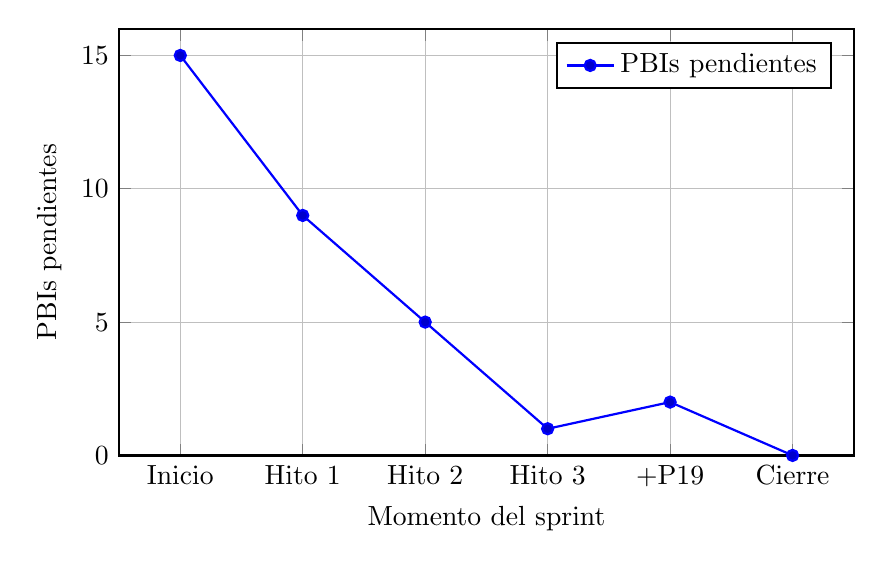
\begin{tikzpicture}
\begin{axis}[
    width=0.9\textwidth,
    height=7cm,
    xlabel={Momento del sprint},
    ylabel={PBIs pendientes},
    xtick={1,2,3,4,5,6},
    xticklabels={Inicio, Hito 1, Hito 2, Hito 3, +P19, Cierre},
    ymin=0, ymax=16,
    grid=major,
    legend pos=north east,
    mark=*,
    thick
]
\addplot coordinates {(1,15) (2,9) (3,5) (4,1) (5,2) (6,0)};
\addlegendentry{PBIs pendientes}
\end{axis}
\end{tikzpicture}
\caption{Burndown del Sprint 1: evolución de PBIs pendientes del alcance de la entrega.}
\label{fig:burndown-s1}
\end{figure}

\subsubsection{Seguimiento visual en DoneTonic}
La Figura \ref{fig:donetonic-graficas-s1} muestra las gráficas Sprint Burnup y Sprint Burndown de DoneTonic para el Sprint 1 (captura \texttt{figs/capturas/donetonic/02-graficas-sprint.png}).

\begin{figure}[htbp]
\centering
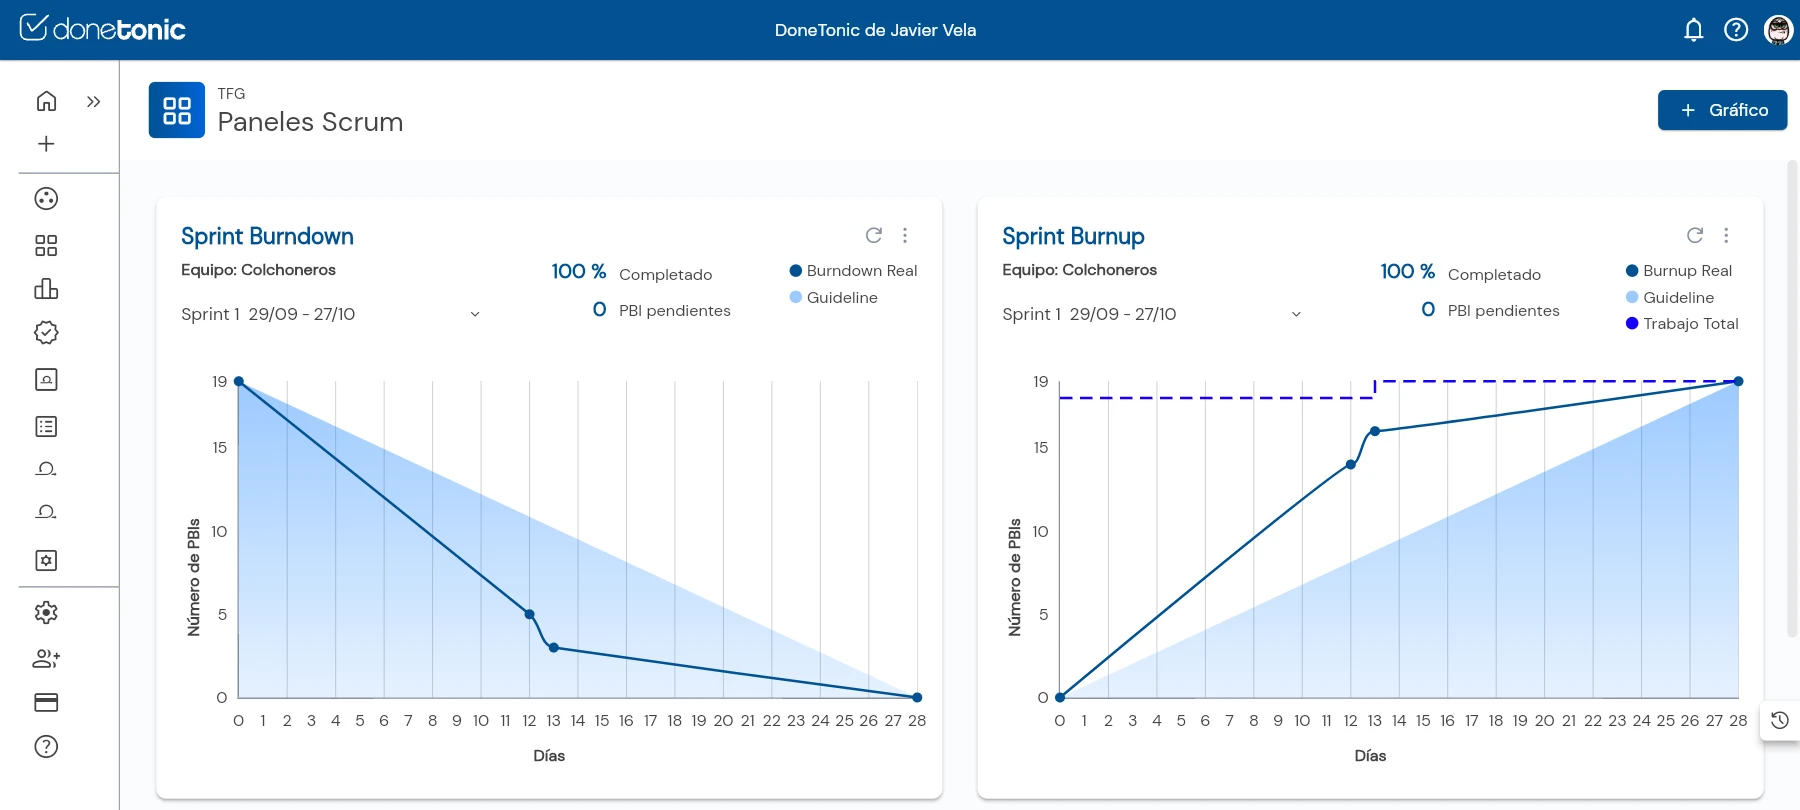
\includegraphics[width=0.9\textwidth]{figs/capturas/donetonic/02-graficas-sprint.png}
\caption{Sprint Burnup y Sprint Burndown en DoneTonic (Sprint 1).}
\label{fig:donetonic-graficas-s1}
\end{figure}

\subsubsection{Cambio de alcance}
Durante el sprint, el profesor repartió créditos de Google Cloud para educación. Para aprovecharlos se añadió el PBI \textbf{P19} (despliegue continuo en Google Cloud Run) con sus tareas T29 y T30. Render se mantuvo como despliegue alternativo. Este cambio se refleja en el burndown como un incremento temporal de PBIs pendientes (de 1 a 2) antes del cierre final.

\subsubsection{Lo aprendido}
\begin{itemize}
    \item La disciplina de GitHub Flow (rama por tarea, PR, CI obligatorio) garantiza que no se integra código roto, pero exige sincronización continua de ramas locales para evitar conflictos de avance rápido.
    \item El patrón repositorio con inyección de dependencias permitió sustituir el almacenamiento en memoria por PostgreSQL sin modificar una sola línea de la capa de lógica, respaldado por pruebas de contrato idénticas.
    \item La auditoría manual frase a frase frente al enunciado oficial demostró ser indispensable, localizando discrepancias de acceso que habían pasado inadvertidas en la formulación de los PBIs.
    \item La concentración cronológica de commits en una jornada (12/10/2026) preserva la trazabilidad estructural del proceso, si bien se reconoce la conveniencia pedagógica de una cadencia temporal más distribuida.
    \item Todo secreto compartido involuntariamente en canales de comunicación debe ser rotado como buena práctica de seguridad.
\end{itemize}

\section{Sprint 2 (Lógica del juego)}

\subsection{Planificación del Sprint 2}

\subsubsection{Objetivo y fechas}
El Sprint 2 se planificó del 23/10/2026 al 29/10/2026, tras el cierre del Sprint 1, cuando el profesor fijó que el Sprint 2 sería la lógica del juego. El juego ya estaba desarrollado en seis fases (23/10–26/10), por lo que el sprint recoge ese trabajo como backlog: 29 PBIs (P20–P48) y 50 tareas (T33–T82), con una etiqueta por fase (gestion/README.md §4.4).

\subsubsection{Sprint Backlog}
La Tabla \ref{tab:sprint2-backlog} resume los PBIs del Sprint 2 con su etiqueta, título, tareas, PRs y fecha de finalización (hecho = día fusión último PR del PBI).

{\small
\begin{longtable}{@{}L{0.7cm} L{2.2cm} L{5.5cm} L{1.5cm} L{2.0cm} L{1.8cm} L{1.5cm}@{}}
\caption{Sprint Backlog del Sprint 2 (29 PBIs, 50 tareas).}\label{tab:sprint2-backlog}\\
\toprule
\textbf{PBI} & \textbf{Etiqueta} & \textbf{Título} & \textbf{Tareas} & \textbf{PRs} & \textbf{Hecho} & \textbf{Estado} \\ \midrule \endfirsthead
\toprule
\textbf{PBI} & \textbf{Etiqueta} & \textbf{Título} & \textbf{Tareas} & \textbf{PRs} & \textbf{Hecho} & \textbf{Estado} \\ \midrule \endhead
P20 & Base del juego & Rediseño interfaz web y menú juego & T33, T34 & \#36, \#45 & 24/10/2026 & Hecho \\
P21 & Base del juego & Motor partida survivor & T35, T36 & \#36 & 23/10/2026 & Hecho \\
P22 & Base del juego & Gráficos pixel art y cámara 3/4 & T37, T38 & \#44, \#46 & 24/10/2026 & Hecho \\
P23 & Base del juego & Jugadores, entrenadores y Vestuario & T39–T41 & \#44, \#48 & 24/10/2026 & Hecho \\
P24 & Base del juego & Armas, habilidades y mejoras & T42, T43 & \#36, \#48 & 24/10/2026 & Hecho \\
P25 & Base del juego & Rivales con comportamiento propio & T44, T45 & \#44, \#45, \#47 & 24/10/2026 & Hecho \\
P26 & Base del juego & Jefes con fases & T46, T47 & \#45, \#48 & 24/10/2026 & Hecho \\
P27 & Base del juego & Mapa con terreno y obstáculos & T48, T49 & \#45, \#47 & 24/10/2026 & Hecho \\
P28 & Base del juego & Controles, pantalla completa y ajustes & T50, T51 & \#36, \#47 & 24/10/2026 & Hecho \\
P29 & Fase 2 Club & Progreso juego guardado en servidor & T52, T53 & \#49 & 24/10/2026 & Hecho \\
P30 & Fase 2 Club & Contratos: fichar jugadores & T54 & \#49 & 24/10/2026 & Hecho \\
P31 & Fase 2 Club & Entrenamiento de jugadores & T55 & \#49, \#50 & 24/10/2026 & Hecho \\
P32 & Fase 2 Club & Ranking de la grada & T56 & \#49 & 24/10/2026 & Hecho \\
P33 & Fase 3 Ultras & Combinaciones y ULTRAS & T57, T58 & \#50 & 24/10/2026 & Hecho \\
P34 & Fase 3 Ultras & Dificultad equilibrada y modo pruebas & T59, T60 & \#50 & 24/10/2026 & Hecho \\
P35 & Fase 4 Mundo & Mundo procedural natural & T61 & \#52 & 24/10/2026 & Hecho \\
P36 & Fase 4 Mundo & Ambientes por finales & T62 & \#52 & 24/10/2026 & Hecho \\
P37 & Fase 4 Mundo & Mote y avatar & T63 & \#52 & 24/10/2026 & Hecho \\
P38 & Fase 5 Rarezas & Rarezas por historia rojiblanca y fichajes & T64, T65 & \#53 & 26/10/2026 & Hecho \\
P39 & Fase 5 Rarezas & Habilidades niveladas por minuto & T66 & \#53 & 26/10/2026 & Hecho \\
P40 & Fase 5 Rarezas & Combinaciones y ultras a la vista & T67 & \#53 & 26/10/2026 & Hecho \\
P41 & Fase 5 Rarezas & Colisiones exactas & T68 & \#53 & 26/10/2026 & Hecho \\
P42 & Fase 6 Logros y sonido & Logros con historia y equipaciones & T69, T70 & \#54 & 26/10/2026 & Hecho \\
P43 & Fase 6 Logros y sonido & Pantalla fin con estadísticas & T71 & \#54 & 26/10/2026 & Hecho \\
P44 & Fase 6 Logros y sonido & Música chiptune y grada & T72–T74 & \#54 & 26/10/2026 & Hecho \\
P45 & Fase 6 Logros y sonido & Muñecos con más detalle & T75 & \#54 & 26/10/2026 & Hecho \\
P46 & Fase 6 Logros y sonido & Jefes más duros & T76 & \#54 & 26/10/2026 & Hecho \\
P47 & Calidad & Corrección errores detectados & T77–T79 & \#51, \#55, \#56 & 29/10/2026 & Hecho \\
P48 & Calidad & Documentación y gestión Sprint 2 & T80–T82 & \#55 & 29/10/2026 & Hecho \\
\bottomrule
\end{longtable}
}

La Tabla \ref{tab:sprint2-backlog} muestra el desglose completo.

\subsubsection{Historias de usuario y criterios de aceptación (Sprint 2)}
Cada PBI del Sprint 2 tiene en DoneTonic su historia de usuario y criterios de aceptación (gestion/README.md, sección «Historias de usuario y criterios de aceptación»). La Tabla \ref{tab:sprint2-hu} resume las 29 historias con sus criterios principales.

{\small
\begin{longtable}{@{}L{0.7cm} L{13.5cm}@{}}
\caption{Historias de usuario Sprint 2 (resumen).}\label{tab:sprint2-hu}\\
\toprule
\textbf{PBI} & \textbf{Historia de usuario y criterios clave} \\ \midrule \endfirsthead
\toprule
\textbf{PBI} & \textbf{Historia de usuario y criterios clave} \\ \midrule \endhead
P20 & Como aficionado quiero una web con aspecto de juego, clara en móvil y ordenador, para que entrar a jugar sea lo primero que vea al iniciar sesión. Criterios: sistema de diseño propio, modo oscuro rojiblanco, responsive, menú de juego como inicio con sesión. \\
P21 & Como jugador quiero una partida de supervivencia contra oleadas infinitas, armas automáticas y elección de mejoras al subir de nivel. Criterios: simulación determinista paso fijo 1/60 s, oleadas cada 30 s, experiencia, 3 mejoras aleatorias, dificultad creciente, pausa y fin de partida. \\
P22 & Como jugador quiero estilo visual propio con muñecos chibi del Atleti generados por código. Criterios: muñecos 16×20 px en canvas, caché de fotogramas, cámara 3/4 con inercia, respeta prefers-reduced-motion. \\
P23 & Como jugador quiero elegir entre 36 futbolistas por posición y 2 entrenadores con ulti. Criterios: stats base por posición, rasgos y habilidades propias por jugador, 2 entrenadores con bonus y ulti, Vestuario con filtro y ficha. \\
P24 & Como jugador quiero 24 armas/habilidades con 5 niveles, pasivas y mejoras extra. Criterios: armas disparo y melé, 5 niveles, pasivas, mejoras extra sin límite, porteros sin armas de disparo. \\
P25 & Como jugador quiero 16 equipos rivales con comportamientos variados. Criterios: 16 equipos desbloqueables por oleadas, arquetipos embestida/disparo, rodean obstáculos, élites blindado/veloz/furioso. \\
P26 & Como jugador quiero 10 jefes con 3 fases, avisos, escolta y jugada estrella. Criterios: jefe cada 4 oleadas, 3 fases (66\%, 33\%), escolta desde 2º jefe, furia por tiempo, jugada estrella en fase 3. \\
P27 & Como jugador quiero mapa procedural con biomas, barro, lluvia, gradas, mesetas. Criterios: ruido armónico continuo, distritos, gradas orientadas, plazas, barro/lluvia, mesetas con escaleras, casi todo alcanzable. \\
P28 & Como jugador quiero controles teclado, ratón, táctil, pausa, pantalla completa, ajustes. Criterios: WASD/flechas, joystick táctil, F pantalla completa, Esc/P pausa, ajustes guardados en navegador. \\
P29 & Como jugador quiero mi club y partidas guardados en mi cuenta con validación anti-trampas. Criterios: tablas juego\_perfiles y juego\_records, API /api/juego protegida, validación servidor con reloj propio y límites creíbles, concurrencia optimista. \\
P30 & Como jugador quiero ganar fichas de contrato venciendo jefes y canjearlas por jugadores. Criterios: plantilla inicial 4 comunes, 1 ficha por 3 jefes, sorteo ponderado por rareza, sin repetir jugador. \\
P31 & Como jugador quiero entrenar a mis jugadores con puntos de jefes y bajas. Criterios: puntos por jefes (1 cada 3) y bajas (coste creciente), 4 stats (Vida, Defensa, Disparo, Suerte) máx. 20, validado en servidor. \\
P32 & Como jugador quiero ranking global con la mejor marca de cada aficionado sin mostrar correo. Criterios: una fila por usuario (mejor tiempo, desempate nivel), pestañas Mis partidas / La grada, anonimizado. \\
P33 & Como jugador quiero 24 combinaciones tácticas y 6 ULTRAS automáticas al completar combinaciones. Criterios: 24 sinergias con bonus, 6 ULTRAS (Puskás, Balón de Oro, MVP Champions, Zamora, Bota de Oro, Mejor Mundial), efecto visual y daño porcentual reducido vs jefes. \\
P34 & Como jugador quiero dificultad justa y modo pruebas para admin. Criterios: tramo final duro desde min 9, rivales curtidos min 12, ayuda inicial 8 min, modo pruebas admin (desbloqueo sin tocar ranking). \\
P35 & Como jugador quiero mundo procedural natural con distritos, estadios, plazas, mesetas. Criterios: ruidos suaves continuos, gradas orientadas, plazas con tiendas, mesetas con escaleras, casi todo alcanzable (test). \\
P36 & Como jugador quiero 5 ambientes que cambien cada 5 min (pretemporada → Copa → Liga → Champions → Mundial). Criterios: cambio de luz, césped, afición, carteles, rivales más fuertes, camisetas de selección en Mundial. \\
P37 & Como jugador quiero mote único y avatar propio en cabecera y ranking. Criterios: mote 3-16 chars único normalizado (sin mayúsculas/tildes), avatar de jugador/entrenador fichado, migración 004, PUT /api/juego/identidad. \\
P38 & Como aficionado quiero rarezas según historia rojiblanca y animación de firma al fichar. Criterios: 4 rarezas (Común 12, Raro 8, Épico 8, Leyenda 8) por historia en el club, más rareza = más habilidades y menos probabilidad, animación firma pixel art. \\
P39 & Como jugador quiero que habilidades fuertes no salgan al principio. Criterios: niveles bloqueados por minuto (desdeMinuto) y recarga mínima (cdMin), regate/entrada/contragolpe reequilibrados. \\
P40 & Como jugador quiero ver combinaciones y ULTRAS con filtros. Criterios: pantalla Combinaciones con nombre, bonus, requisitos, ultra asociada, filtros Todas/Con tu jugador/Conseguidas. \\
P41 & Como jugador quiero colisiones exactas (lo que se ve choca). Criterios: hitbox por los pies (vista 3/4), obstáculos macizos en todo su dibujo, copa de árboles transparente. \\
P42 & Como aficionado quiero 29 logros con datos históricos que desbloqueen 10 equipaciones. Criterios: 29 logros con dato real, servidor valida los comprobables, 10 equipaciones en Vestuario. \\
P43 & Como jugador quiero pantalla de fin con desglose de daño por arma y recompensas. Criterios: tiempo, ambiente, bajas, jefes, daño total, golpe máx, críticos, daño recibido, vida recuperada, barras por arma/ultra/ulti/quemaduras, logros nuevos. \\
P44 & Como jugador quiero música chiptune, fanfarrias y grada con volumen independiente. Criterios: secuenciador chiptune propio, canción por ambiente que anima con tiempo/jefes, fanfarria por competición, grada con murmullo/cánticos según distancia, todo Web Audio sin archivos. \\
P45 & Como aficionado quiero reconocer jugadores y jefes en el campo. Criterios: sombreado, orejas, nariz, peinados, rasgos propios (brazalete, cinta, pecas, barba, pendientes, tatuajes). \\
P46 & Como jugador quiero jefes más duros a partir del segundo. Criterios: escolta de élites desde 2º jefe, refuerzos al cambiar fase, furia si tardas, jugada estrella en fase 3, 1º jefe asequible. \\
P47 & Como usuario quiero que los errores encontrados se arreglen con pruebas de regresión. Criterios: cada error reproducido con prueba antes de arreglar, arreglos pasan CI y se despliegan. \\
P48 & Como responsable quiero todo el Sprint 2 revisable desde el repo. Criterios: README con capturas juego y DoneTonic, documentación técnica para memoria, backlog/tablero/gráficas Sprint 2 en DoneTonic. \\
\bottomrule
\end{longtable}
}

La Tabla \ref{tab:sprint2-hu} condensa las 29 historias de usuario del Sprint 2.

\subsubsection{Trazabilidad}
Las tareas de cada PBI indican en su descripción de DoneTonic el PR donde está el trabajo. La Tabla \ref{tab:sprint2-trazabilidad} muestra la correspondencia tarea → PR.

{\small
\begin{longtable}{@{}L{0.7cm} L{1.0cm} L{5.5cm} L{3.0cm} L{2.5cm}@{}}
\caption{Trazabilidad tarea → PR del Sprint 2 (50 tareas).}\label{tab:sprint2-trazabilidad}\\
\toprule
\textbf{PBI} & \textbf{Tarea} & \textbf{Descripción} & \textbf{PR} & \textbf{Estado} \\ \midrule \endfirsthead
\toprule
\textbf{PBI} & \textbf{Tarea} & \textbf{Descripción} & \textbf{PR} & \textbf{Estado} \\ \midrule \endhead
P20 & T33 & Sistema de diseño: tokens, tipografía y modo oscuro rojiblanco & \#36 & Hecho \\
P20 & T34 & Menú del juego como inicio con sesión (hub con jugador paseando) & \#36, \#45 & Hecho \\
P21 & T35 & Simulación de paso fijo con semilla (mundo.js) & \#36 & Hecho \\
P21 & T36 & Oleadas, experiencia y mejoras al subir de nivel & \#36 & Hecho \\
P22 & T37 & Muñecos chibi generados por código (sprites.js) & \#44 & Hecho \\
P22 & T38 & Cámara 3/4, inercia y sensación de movimiento y golpes & \#46 & Hecho \\
P23 & T39 & Jugadores con estadísticas por posición y habilidades propias & \#44, \#48 & Hecho \\
P23 & T40 & Entrenadores con ulti y pantalla Dirección & \#44 & Hecho \\
P23 & T41 & Vestuario renovado con filtros y ficha & \#48 & Hecho \\
P24 & T42 & Armas con 5 niveles: disparo, cuerpo a cuerpo y movilidad & \#36, \#48 & Hecho \\
P24 & T43 & Pasivas y mejoras extra & \#36 & Hecho \\
P25 & T44 & 16 equipos rivales que se desbloquean por oleadas & \#44 & Hecho \\
P25 & T45 & Rivales que embisten, disparan y rodean obstáculos & \#45, \#47 & Hecho \\
P26 & T46 & Jefes con tres fases y avisos de ataque & \#45 & Hecho \\
P26 & T47 & Seis jefes nuevos con habilidades propias & \#48 & Hecho \\
P27 & T48 & Barro, lluvia, gradas y premios & \#45 & Hecho \\
P27 & T49 & Mapa procedural con biomas y estructuras & \#47 & Hecho \\
P28 & T50 & Entrada por teclado y joystick táctil & \#36 & Hecho \\
P28 & T51 & Pantalla completa, pausa y ajustes en partida & \#47 & Hecho \\
P29 & T52 & Migración 003 y repositorios del juego (memoria y PostgreSQL) & \#49 & Hecho \\
P29 & T53 & API del juego con validación anti-trampas & \#49 & Hecho \\
P30 & T54 & Fichas por jefes y sorteo de contratos por rareza & \#49 & Hecho \\
P31 & T55 & Puntos y estadísticas de entrenamiento & \#49, \#50 & Hecho \\
P32 & T56 & Ranking multijugador con la mejor partida de cada usuario & \#49 & Hecho \\
P33 & T57 & Combinaciones con nombre y bonus & \#50 & Hecho \\
P33 & T58 & Seis ULTRAS con efectos visuales & \#50 & Hecho \\
P34 & T59 & Curvas de dificultad calibradas con un bot & \#50 & Hecho \\
P34 & T60 & Modo pruebas para administradores & \#50 & Hecho \\
P35 & T61 & Generación del terreno por ruidos (terreno.js) & \#52 & Hecho \\
P36 & T62 & Cinco ambientes con cambio de luz, afición y fuerza & \#52 & Hecho \\
P37 & T63 & Migración 004, API de identidad y pantalla Tu ficha & \#52 & Hecho \\
P38 & T64 & Rarezas por historia y 36 jugadores & \#53 & Hecho \\
P38 & T65 & Animación de la firma del contrato & \#53 & Hecho \\
P39 & T66 & Niveles bloqueados por minuto y recarga mínima & \#53 & Hecho \\
P40 & T67 & Pantalla de combinaciones y ultras con filtros & \#53 & Hecho \\
P41 & T68 & Hitbox por los pies y obstáculos macizos & \#53 & Hecho \\
P42 & T69 & Logros validados en el servidor (logros.js) & \#54 & Hecho \\
P42 & T70 & Pantalla Logros y equipaciones en el Vestuario & \#54 & Hecho \\
P43 & T71 & Atribución del daño por fuente y pantalla de fin (fin-ui.js) & \#54 & Hecho \\
P44 & T72 & Secuenciador chiptune y fanfarrias (musica.js) & \#54 & Hecho \\
P44 & T73 & La grada: murmullo y cánticos según la cercanía & \#54 & Hecho \\
P44 & T74 & Efectos de sonido nuevos y ajuste de música & \#54 & Hecho \\
P45 & T75 & Rasgos y sombreado en sprites.js & \#54 & Hecho \\
P46 & T76 & Escolta, furia y jugada estrella & \#54 & Hecho \\
P47 & T77 & El juego no cargaba (variable usada antes de existir) & \#51 & Hecho \\
P47 & T78 & El primer clic en «Reenviar el correo» se perdía tras un error & \#55 & Hecho \\
P47 & T79 & No se podía volver tras eliminar la cuenta (Google) & \#56 & Hecho \\
P48 & T80 & README del Sprint 2 con capturas del juego y de DoneTonic & \#55 & Hecho \\
P48 & T81 & Documentación técnica para la memoria & \#55 & Hecho \\
P48 & T82 & Backlog y seguimiento del Sprint 2 en DoneTonic & — (DoneTonic) & Hecho \\
\bottomrule
\end{longtable}
}

La Tabla \ref{tab:sprint2-trazabilidad} detalla las 50 tareas del Sprint 2.

\subsection{Desarrollo del Sprint 2: problemas y soluciones}

Los problemas detectados durante el Sprint 2 y sus soluciones (documentacion-tecnica.md §13) se recogen en la Tabla \ref{tab:prob-sprint2}.

\begin{longtable}{@{}L{5.5cm} L{8.5cm}@{}}
\caption{Problemas y soluciones del Sprint 2.}\label{tab:prob-sprint2}\\
\toprule
\textbf{Problema detectado} & \textbf{Solución adoptada} \\ \midrule \endfirsthead
\toprule
\textbf{Problema detectado} & \textbf{Solución adoptada} \\ \midrule \endhead
El juego dejó de cargar tras un cambio (variable usada antes de existir) & Arreglo inmediato (PR \#51) y prueba que importa todos los módulos del juego \\
Jugadores podían esconderse detrás de tejados (colisión no coincidía con dibujo 3/4) & Colisión por los pies y obstáculos macizos en todo su dibujo (PR \#53) \\
Tirones al pintar el suelo (muchas texturas por píxel en mismo fotograma) & Una textura por celda y ambiente, como mucho una por fotograma y por adelantado (PR \#52) \\
Simulación lenta con muchos rivales (búsqueda claves texto) & Búsqueda por radio con claves numéricas empaquetadas: 4,5× más rápido (PR \#52) \\
Regate hacía al jugador intocable demasiado pronto (subía sin límite) & Niveles bloqueados por minuto (desdeMinuto) y recarga mínima (cdMin) (PR \#53) \\
Equilibrio difícil de ajustar a mano (muchas variables) & Todo el equilibrio en config.js y calibración con bot que juega partidas simuladas (PR \#50) \\
Eliminar cuenta (especialmente Google) impedía volver a entrar con ese email & Migración 005: índice parcial unique en email (solo cuentas no eliminadas), findByEmail ignora eliminadas, suelta mote y sale del ranking (PR \#56) \\
Primer clic en «Reenviar el correo» se perdía tras error de login & Campo vacío sin tocar no da error al salir; tras fallo servidor se vacía contraseña sin marcar error (PR \#55) \\
\bottomrule
\end{longtable}

La Tabla \ref{tab:prob-sprint2} resume los 8 problemas principales del Sprint 2.

\subsection{Revisión del Sprint 2}

Al cierre del Sprint 2 (29/10/2026) se entregaron:
\begin{itemize}
    \item 29 PBIs completados (P20–P48).
    \item 50 tareas cerradas (T33–T82).
    \item 14 PRs fusionados (\#36, \#44–\#56).
    \item Batería de 276 pruebas automatizadas (136 del juego) validadas en CI contra PostgreSQL 17.
    \item Documentación técnica actualizada (documentacion-tecnica.md) y README con capturas del juego y DoneTonic.
    \item Backlog, tablero y gráficas del Sprint 2 registrados en DoneTonic.
\end{itemize}

\subsection{Retrospectiva del Sprint 2}

\subsubsection{Burndown real del Sprint 2}
La Figura \ref{fig:burndown-s2} muestra la evolución real de PBIs pendientes según la fecha de fusión del último PR de cada PBI (tabla «Evolución del Sprint 2» en gestion/README.md). A diferencia de las gráficas de DoneTonic (que salen en recta porque el backlog se registró al cerrar el sprint el 29/10), este burndown refleja el trabajo real día a día.

\begin{figure}[htbp]
\centering
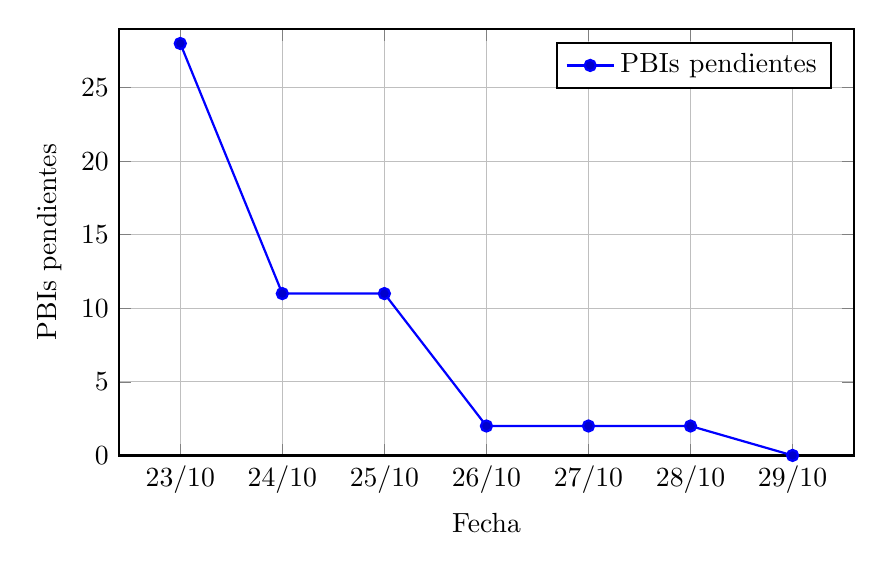
\begin{tikzpicture}
\begin{axis}[
    width=0.9\textwidth,
    height=7cm,
    xlabel={Fecha},
    ylabel={PBIs pendientes},
    xtick={1,2,3,4,5,6,7},
    xticklabels={23/10, 24/10, 25/10, 26/10, 27/10, 28/10, 29/10},
    ymin=0, ymax=29,
    grid=major,
    legend pos=north east,
    mark=*,
    thick
]
\addplot coordinates {(1,28) (2,11) (3,11) (4,2) (5,2) (6,2) (7,0)};
\addlegendentry{PBIs pendientes}
\end{axis}
\end{tikzpicture}
\caption{Burndown real del Sprint 2 (PBIs pendientes según fechas de PR).}
\label{fig:burndown-s2}
\end{figure}

\subsubsection{Seguimiento visual en DoneTonic}
Las Figuras \ref{fig:donetonic-tablero-s2}, \ref{fig:donetonic-graficas-s2} y \ref{fig:donetonic-backlog} muestran el tablero, las gráficas Sprint Burndown/Burnup y el Backlog Burndown/Burnup del Sprint 2 en DoneTonic (capturas 04, 06 y 07 de donetonic).

\begin{figure}[htbp]
\centering
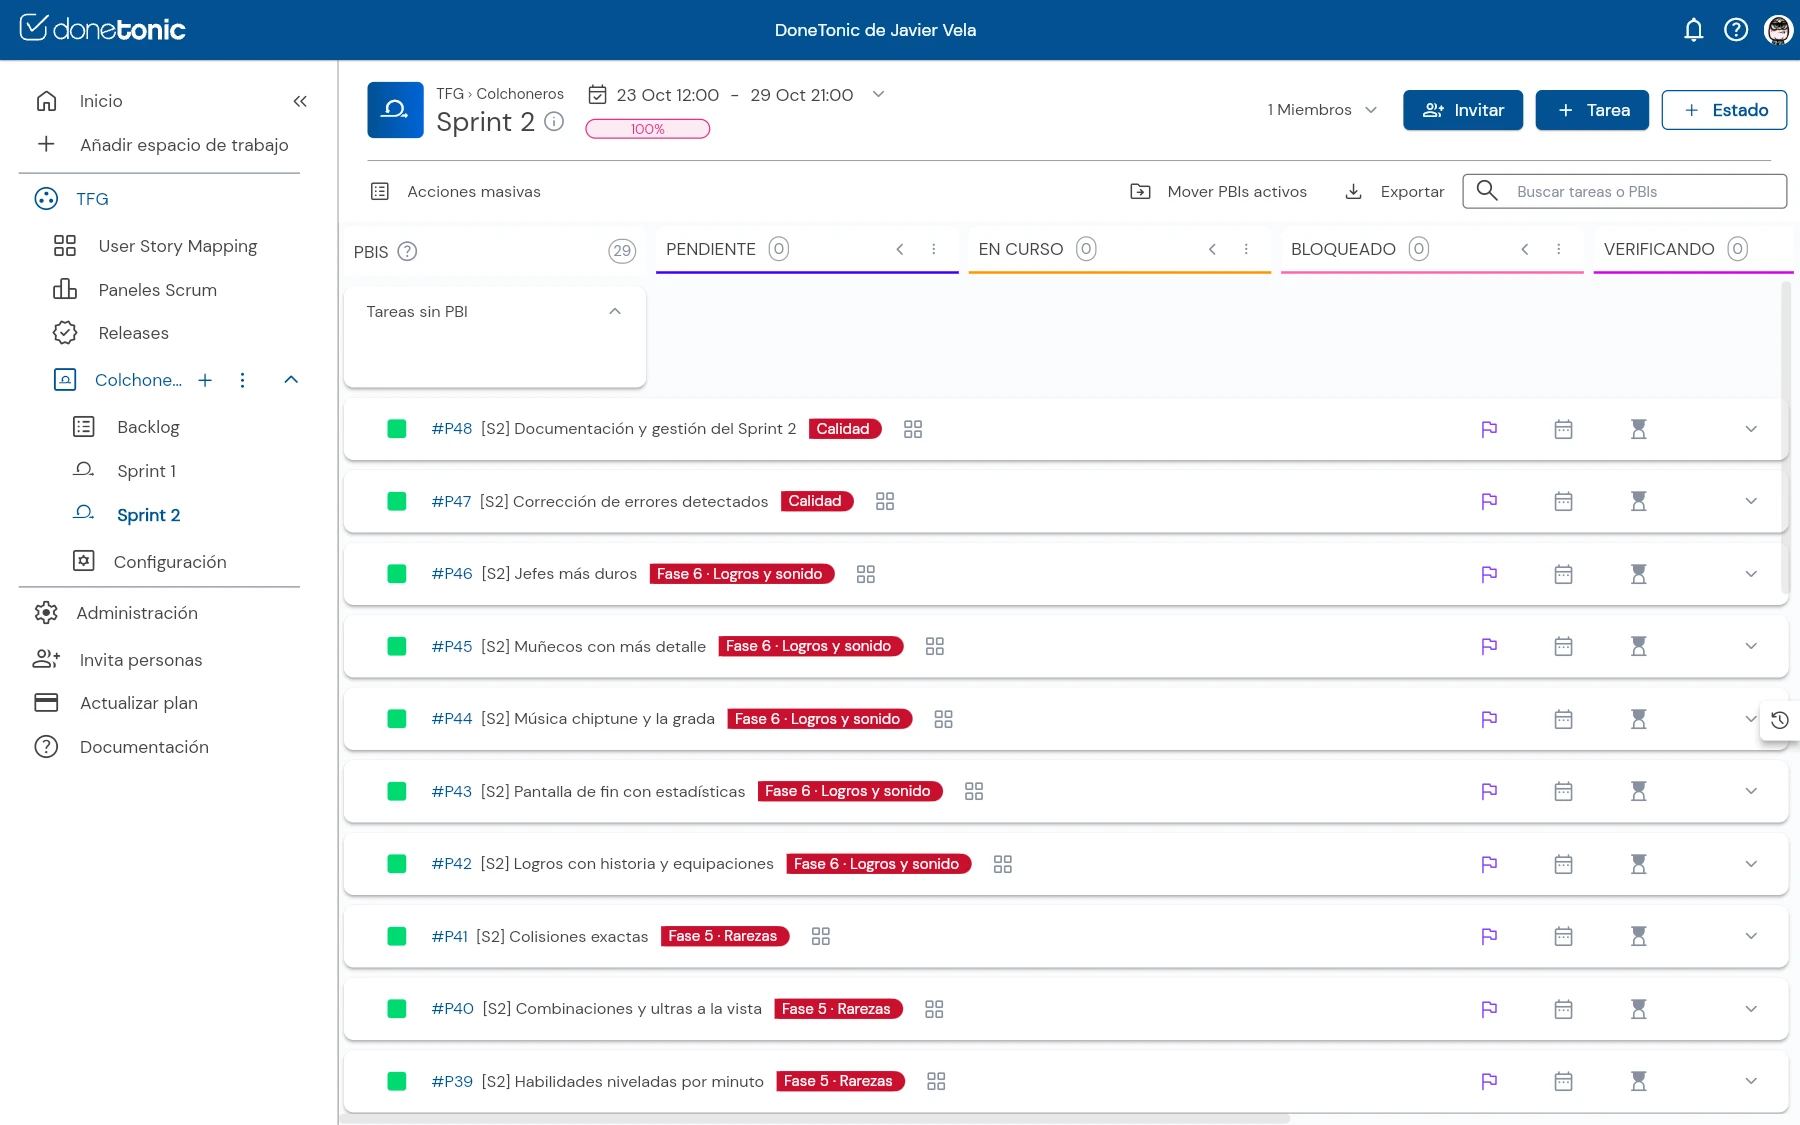
\includegraphics[width=0.9\textwidth]{figs/capturas/donetonic/04-tablero-sprint2.png}
\caption{Tablero del Sprint 2 en DoneTonic al 100\%.}
\label{fig:donetonic-tablero-s2}
\end{figure}

\begin{figure}[htbp]
\centering
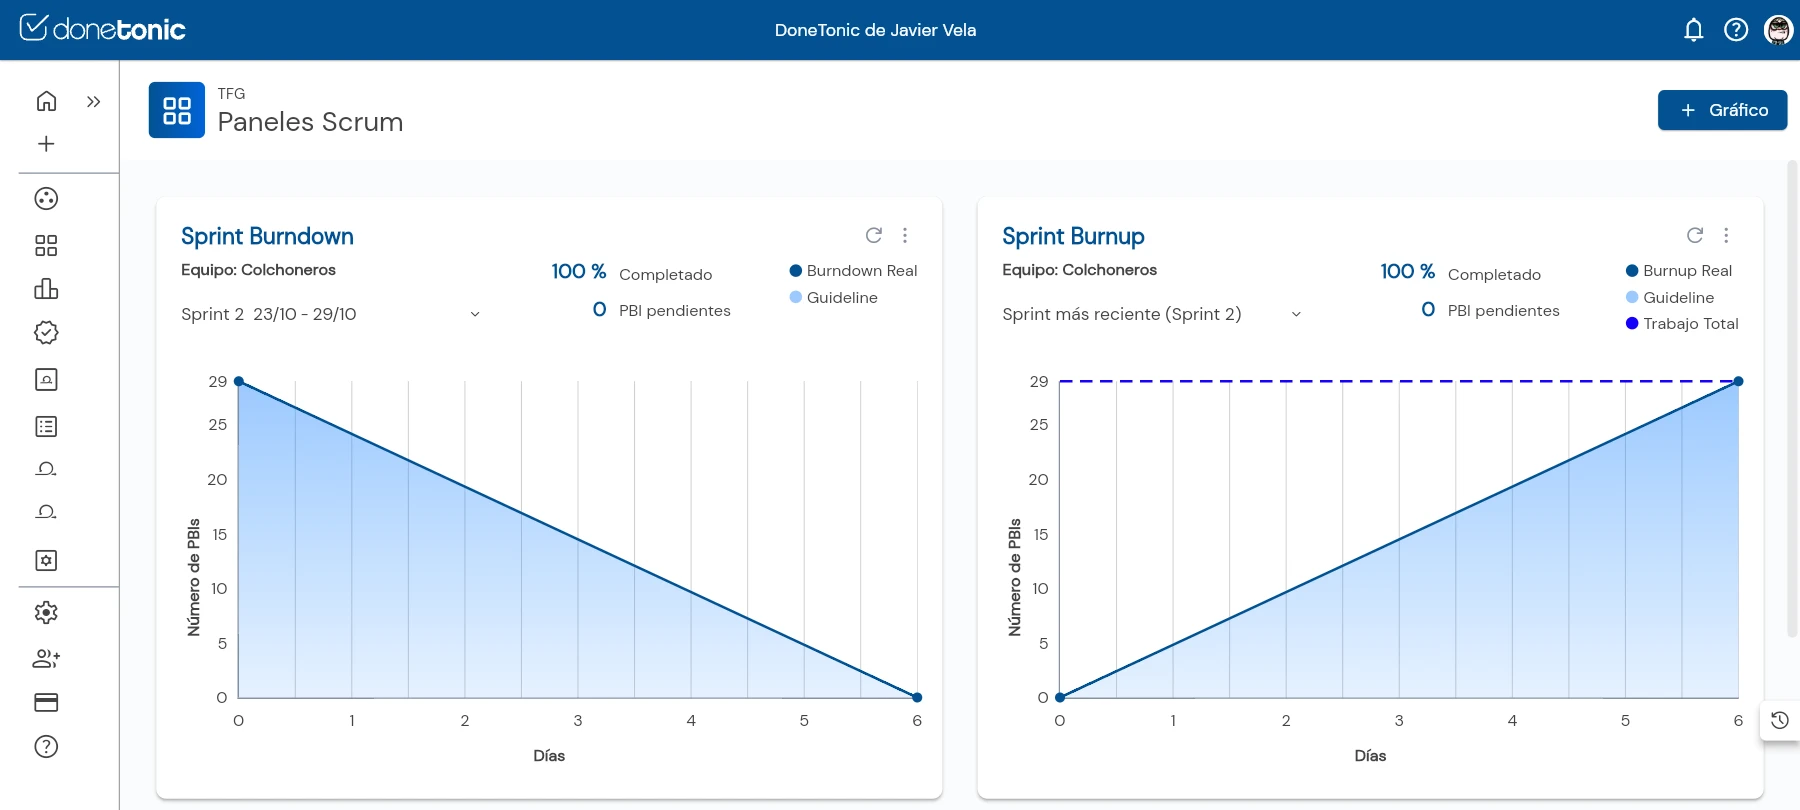
\includegraphics[width=0.9\textwidth]{figs/capturas/donetonic/06-graficas-sprint2.png}
\caption{Sprint Burndown y Burnup del Sprint 2 en DoneTonic (aplanadas por registro tardío).}
\label{fig:donetonic-graficas-s2}
\end{figure}

\begin{figure}[htbp]
\centering
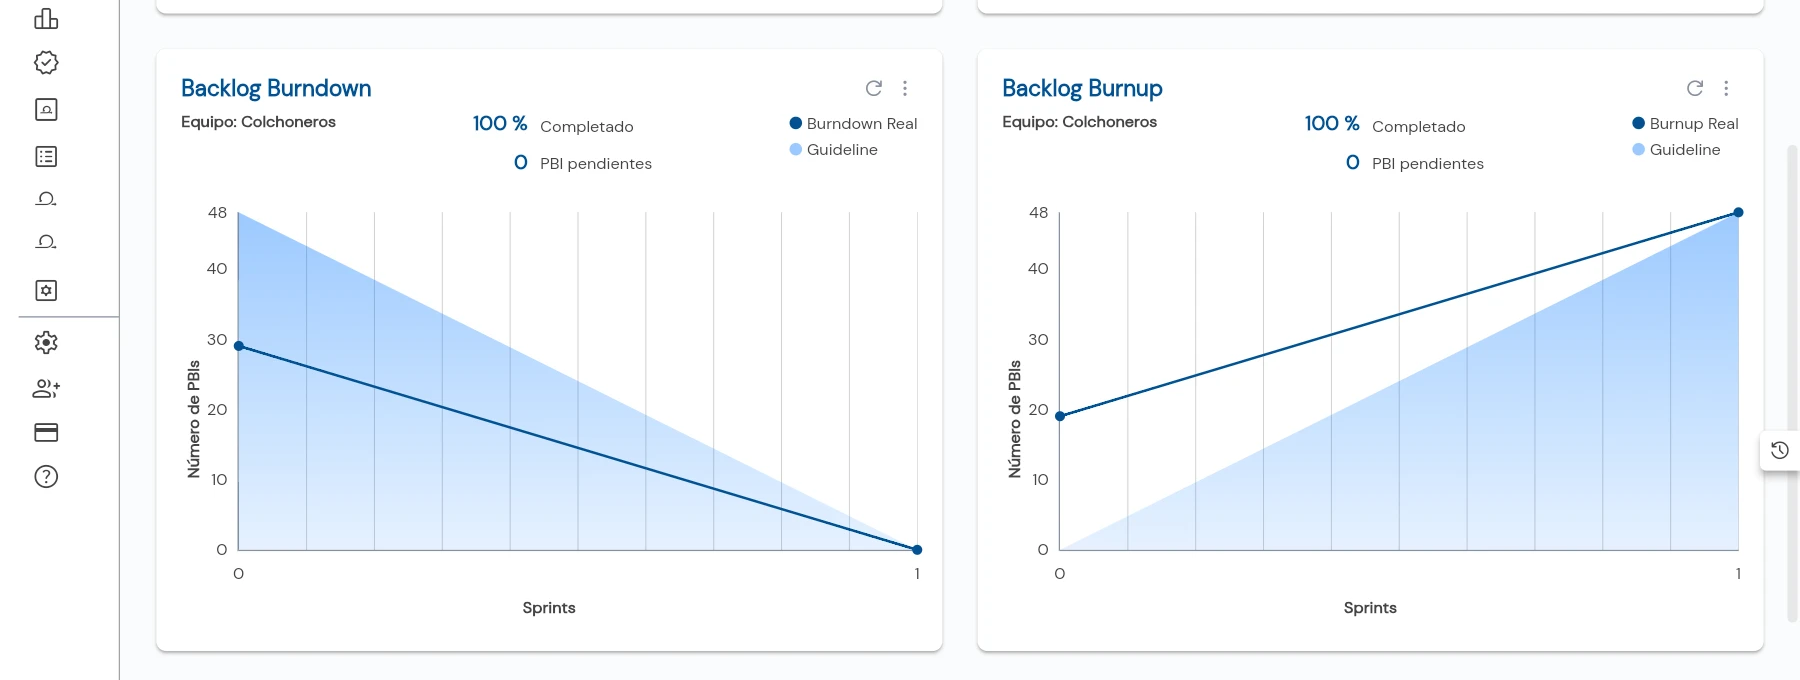
\includegraphics[width=0.9\textwidth]{figs/capturas/donetonic/07-graficas-backlog.png}
\caption{Backlog Burndown y Burnup de los dos sprints en DoneTonic.}
\label{fig:donetonic-backlog}
\end{figure}

\subsubsection{Explicación de las gráficas planas en DoneTonic}
Como se indica en la Figura \ref{fig:donetonic-graficas-s2}, las gráficas de DoneTonic del Sprint 2 aparecen como una recta porque el backlog completo (29 PBIs, 50 tareas) se registró en la herramienta el 29/10/2026, al cerrar el sprint, marcando todos los PBIs como hechos ese mismo día. La evolución real del trabajo (del 23 al 26/10) se reconstruye a partir de las fechas de fusión de los PRs, como se muestra en la Figura \ref{fig:burndown-s2}.

\subsubsection{Lo aprendido}
\begin{itemize}
    \item La arquitectura en capas y la inyección de dependencias permitieron añadir la lógica del juego (11.000 líneas) sin tocar la base SaaS, reutilizando usuarios, sesiones, roles, persistencia y CI/CD.
    \item La simulación determinista con paso fijo y semilla facilitó las pruebas automáticas del motor (136 pruebas) y la validación anti-trampas en el servidor.
    \item La generación procedural de gráficos y audio por código eliminó dependencias de assets externos y permitió variaciones dinámicas (equipaciones, selecciones, intensidad musical).
    \item La concurrencia optimista (columna \texttt{version} en \texttt{juego\_perfiles}) resolvió condiciones de carrera al fichar/entrenar sin bloqueos pesados.
    \item El registro tardío en DoneTonic distorsiona las métricas visuales; para retrospectivas reales hay que cruzar con fechas de PR/commits.
\end{itemize}
